%\documentclass[twocolumn]{emulateapj}
%\documentclass[12pt,preprint]{aastex}

\documentclass[usenatbib]{mn2e}

\newcommand{\s}{$_{\rm s}$}
\newcommand{\kms}{km~s$^{-1}$}
\newcommand{\msun}{{\it M}$_{\odot}$}
\newcommand{\lsun}{{\it L}$_{\odot}$}
\newcommand{\mear}{{\it M}$_{\oplus}$}
\newcommand{\etal}{{\it et al.}}
\newcommand{\ie}{{\it i.e.}}
\newcommand{\eg}{{\it e.g.}}
\newcommand{\be}{\begin{equation}}
\newcommand{\ee}{\end{equation}}
\newcommand{\magarc}{{\rm mag\,arcsec$^{-2}$}}
\newcommand{\MK}{{{\rm M}_{\rm ext,K}-5\log h}}
\newcommand{\ri}{{$r_{21}$}}
\newcommand{\ra}{$R_A$}
\newcommand{\vobs}{{v_{\rm obs}}}
\newcommand{\kmsMpc}{km~s$^{-1}$ Mpc$^{-1}$}
\newcommand{\h}{$h_{70}$}
\newcommand{\vpec}{v_{\rm pec}}
\newcommand{\like}{{\mathcal L}}
\newcommand{\vs}{\vspace*{5pt}}
\newcommand{\continued}{ (Continued)}

% Journals
\newcommand{\mnras}{MNRAS}
\newcommand{\apj}{ApJ}
\newcommand{\apjl}{ApJL}
\newcommand{\aj}{AJ}
\newcommand{\pasp}{PASP}
\newcommand{\aaps}{A\&AS}
\newcommand{\aap}{A\&A}
\newcommand{\apjs}{ApJS}
\newcommand{\araa}{ARA\&A}

\newcommand{\pbar}{p_{\rm bar}}
\newcommand{\fHI}{f_{\rm HI}}

%\shorttitle{Galaxy Zoo View of the Hubble Sequence}
%\shortauthors{Masters \etal}

\voffset-1.25cm

\usepackage{epsfig}
\usepackage{color}
\begin{document}

%\title{The Galaxy Zoo View of the Hubble Sequence}
%\author{Galaxy Zoo Team} 
%\altaffiltext{1}{ICG}
%\altaffiltext{2}{Harvard-Smithsonian Center for Astrophysics, 60 Garden Street, Cambridge, MA 02138}
%\altaffiltext{3}{MIT}
%\altaffiltext{4}{??}
%\email{kmasters@cfa.harvard.edu}

\title[Galaxy Zoo View of the Hubble Sequence]{The Galaxy Zoo View of the Hubble Sequence}
%Bars Regulating Star Formation though the Atomic Gas Content of Disc Galaxies}
%The Atomic Gas Content of Barred Galaxies from ALFALFA$^*$: Bar Feedback in Intermediate Mass Disc Galaxies }
\author[K.L. Masters \etal]{Karen L. Masters$^{1}$, Chris Lintott$^{2}$, Ross Hart$^{3}$, Sandor Kruk$^{2}$, \newauthor Rebecca Smethurst$^{3}$,  Kevin Casteels, Bill Keel, Kyle Willett, ++
\newauthor (order TBD) \\
% Robert C. Nichol$^{1,2}$, Martha P. Haynes$^3$, Chris Lintott$^4$, \newauthor Brooke Simmons$^5$, Ramin Skibba$^6$, Steven Bamford$^7$, Riccardo Giovanelli$^3$, \newauthor  Kevin Schawinski$^{5,8}$ \\
$^1$Institute for Cosmology and Gravitation, University of Portsmouth, Dennis Sciama Building, Burnaby Road, Portsmouth, PO1 3FX, UK \\
%$^2$South East Physics Network, www.sepnet.ac.uk\\
%$^3$Dept. of Astronomy, Cornell University, Space Sciences Building, Ithaca, NY 14850, USA\\
 %$^2$Institute for Sciences of the Cosmos (ICCUB), University of Barcelona, Marti i Franques 1, Barcelona, 08024 Spain\\
 $^{2}$Oxford Astrophysics, Department of Physics, University of Oxford, Denys Wilkinson Building, Keble Road, Oxford, OX1 3RH, UK\\
%$^{5}$Yale Center for Astronomy and Astrophysics, Yale University, P.O. Box 208121, New Haven, CT 06520, USA \\
%$^6$Steward Observatory, University of Arizona, 933 N. Cherry Ave, Tuscon, AZ 85721, USA\\
 %$^4$Astronomy Department, Adler Planetarium and Astronomy Museum, 1300 Lake Shore Drive, Chicago, IL 60605, USA\\
  $^3$Centre for Astronomy \& Particle Theory, University of Nottingham, University Park, Nottingham, NG7 2RD, UK\\
 %$^6$School of Physics and Astronomy, University of Minnesota, Minneapolis, MN 55455, USA\\
 %$^7$Department of Physics \& Astronomy, 206 Gallalee Hall, 514 University Blvd., University of Alabama, Tuscaloosa, AL 35487-0234, USA\\
% $^8$Einstein Fellow\\ 
\\
 $^*$This publication has been made possible by the participation of more than 200,000 volunteers in the Galaxy Zoo project. \\ Their contributions are individually acknowledged at \texttt{http://www.galaxyzoo.org/volunteers}. \\
\\
{\tt E-mail: karen.masters@port.ac.uk}
 }

%\date{Accepted for publication in MNRAS, 7th October 2010.}
%\pagerange{1--10} \pubyear{2010}

\maketitle



\begin{abstract}

We use classifications provided by citizen scientists in the Galaxy Zoo project to give a new perspective on the Hubble Morphological Sequence for galaxies. We demonstrate that the modern use age of the Hubble spiral classifications (Sa--Sd) is based almost entirely on bulge size, with no reference to spiral arm winding, or ``degree of concentration" of the arms, and that furthermore in a volume limited sample of galaxies with both automated and crowdsourced measures of bulge size and spiral arm tightness there is no correlation between the two traditional measures of spiral galaxy type.  

\end{abstract}

%\keywords{galaxies: distances and redshifts --- galaxies: clusters --- galaxies: fundamental parameters --- distance scale --- cosmological parameters}

\section{Introduction}

The classification of objects into categories is a common technique across many areas of science. Galaxy morphology (\ie~ the shapes and features seen in images of galaxies) remains the most common starting point for this process in extragalactic astronomy. %(although classification on the basis of colour or spectral type is also common). 
As a result many galaxy classification schemes have been developed (see Buta 2012, and Sandage 2005 for recent reviews, older reviews which will be of particular interest for historical notes include de Vaucouleurs 1959, Sandage 1975, Buta 1992, Buta, Corwin \& Odewahan 2007). The scheme first presented by Hubble (1926, 1936) remains the basis of the most commonly used classifications (e.g. as used in revised and expanded versions in {\it The Hubble Atlas} by Sandage (1961); or in the Third Reference Catalogue of Bright Galaxies, RC3 by de Vaucouleur (1991)). 

\begin{figure}
\includegraphics[width=84mm]{TuningFork.png}
\caption{The Hubble Sequence illustrated by the examples suggested by Hubble (1926) with images from the SDSS.  The galaxies are: : E0 � NGC 3379; E5 � NGC 4621;  Sa - NGC 4594 (``The Sombrero");  Sb - NGC 2841; Sc -  NGC 5447 (``The Pinwheel"); SBa - NGC 2859; SBb - NGC 3351 (or M95); SBc - 7479. We have also included an S0 (NGC 6278), not in Hubble�s original scheme as no examples were known at the time.) \label{sequence}}
\end{figure}

The basic ``Hubble sequence" splits galaxies into ``spiral" and ``elliptical" types, labelling ellipticals by their degree of elongation (from E0 being completely round, to E7 galaxies, with an ellipticity of 0.7). The spiral galaxies are then ordered in a sequence extending away from the ellipticals,, split into two arms by the presence or absence of a galactic bar (see Figure \ref{sequence} for a schematic using the example galaxies identified by Hubble 1926). Hubble correctly predicted the existence of an intermediate type (lenticulars, or S0s), even through no examples were known at the time (Buta 2012). By analogy with the terminology used for stellar classification (and explicitly making the point that this was not a comment on evolutionary paths\footnote{see the Footnote I on pg 326 of Hubble (1926)}), Hubble dubbed the spiral types (a) ``early",  (b) ``intermediate" and (c) ``late"-type. This appears to be the basis of sometimes confusing terminology which has stuck, with astronomers now more commonly using ``early-type galaxies"  (ETG) to refer to ellitptical and lenticular galaxies (often, but not always, excluding the ``early-type" or Sa spirals, e.g. as used by the ATLAS-3D team; Cappellari et al. 2011a,b); while ``late-type" is commonly used to refer to any spiral galaxies (but sometimes excludes Sa spirals, e.g. Strateva et al 2001).

The morphology of a galaxy encodes information about its formation history and evolution through what it reveals about the orbits of the stars in the galaxy, and is known to correlate remarkably well with other physical properties (e.g. Roberts \& Haynes 1994). These correlations, along with the ease of automated measurement of colour or spectral type, have resulted in a recent trend for classification on the basis of these properties rather than morphology per se (e.g.  Weinmann et al. 2006, van den Bosch et al. 2008, Zehavi et al. 2011). Indeed the strength of the correlation has led some to authors to claim that the correspondance between colour and morphology is so good that that classification by colour alone can be used to replace morphology (e.g. Park \& Choi 2005, Faber et al. 2007). Meanwhile the size of modern data sets (e.g. the Main Galaxy Sample of the Sloan Digital Sky Survey, SDSS, Strauss et al. 2002) made the traditional techniques of morphological classification by small numbers of experts implausible. This problem was solved making use of the technique of crowdsourcing by the Galaxy Zoo project (Lintott et al. 2008, 2011). One of the first results from the Galaxy Zoo morphological classifications was to demonstrate on a firm statistical basis that colour and morphology are not equivalent for all galaxies (Bamford et al. 2009, Schawinski et al. 2009, Masters et al. 2010) and that morphology provides complementary information on galaxy populations useful to understand the processes of galaxy evolution.  

 In this article we explore an updated view of the Hubble Sequence obtained from visual classifications provided by 160,000 members of the public on $\sim$ 250,000 galaxies from the Sloan Digital Sky Survey (SDSS) Main Galaxy Sample (MGS; Strauss et al. 2002). These classifications are described in detail in Willett et al. (2013), available to download from {\tt data.galaxyzoo.org} (as well as being inlucded as an SDSS Value Added Catalogue from DR10 (Ahn et al. 2013) onwards). The basic division into spiral--elliptical (or featured--smooth in the language of Galaxy Zoo, which corresponds to what many astronomers mean by early- and late-type) galaxies has been discussed at length (e.g. Willett et al. 2013). In this article we particularly focus on the spiral (or more precisely ``featured, but not irregular") sequence, and investigate if the traditional criteria for the ordering along this sequence fit in with the picture revealed by Galaxy Zoo morphologies. 

We remind the reader that the original Hubble sequence of Sa-Sb-Sc spiral galaxies (Hubble 1926; and extended to Sd by de Vaucouleurs 1959) was set up using three distinct criteria. These were based on (1) spiral arm appearance, split into (a) how tightly wound the spiral arms are and (b) how clear, or distinct the arms are, and (2) the prominence of the central bulge. Sa galaxies were described as having large bulges and tight, smooth (very distinct) arms, while in contrast a typical Sc was described as having a very small ``inconspicuous" bulge and very loose patchy (indistinct) arms. In Hubble's language ``normal" (S) and ``barred" (SB) spirals had identical parallel sequences. These types are illustrated by the example galaxies given in Hubble (1926; except for the S0 classification which first appeared later) in Figure \ref{sequence}. 

Among experts in morphology (e.g. Sandage 2005, Buta 2012), there has been a consensus that for most spiral galaxies these three criteria result in consistent classification. Buta (2012) explains however, that ``in conflicting cases, emphasis is usually placed on the appearance of the arms". Examples of conflicting cases, particularly of galaxies with tightly wound spirals and small bulges are found in the literature (for example - Sandage 1961, Hogg, Roberts \& Sandage 1993, Sandage \& Bedke (1994), Jore, Broeils \& Haynes 1996, see Figure \ref{Sa}). Sandage (2005) notes that the existence of ``small bulge Sa galaxies" (as defined by their arm types) had been recognised even in Hubble's time. Buta (2012) also explains that SB galaxies with nuclear rings in small bulges may commonly have tightly wound arms, and therefore be classes as Sa. 

\begin{figure}
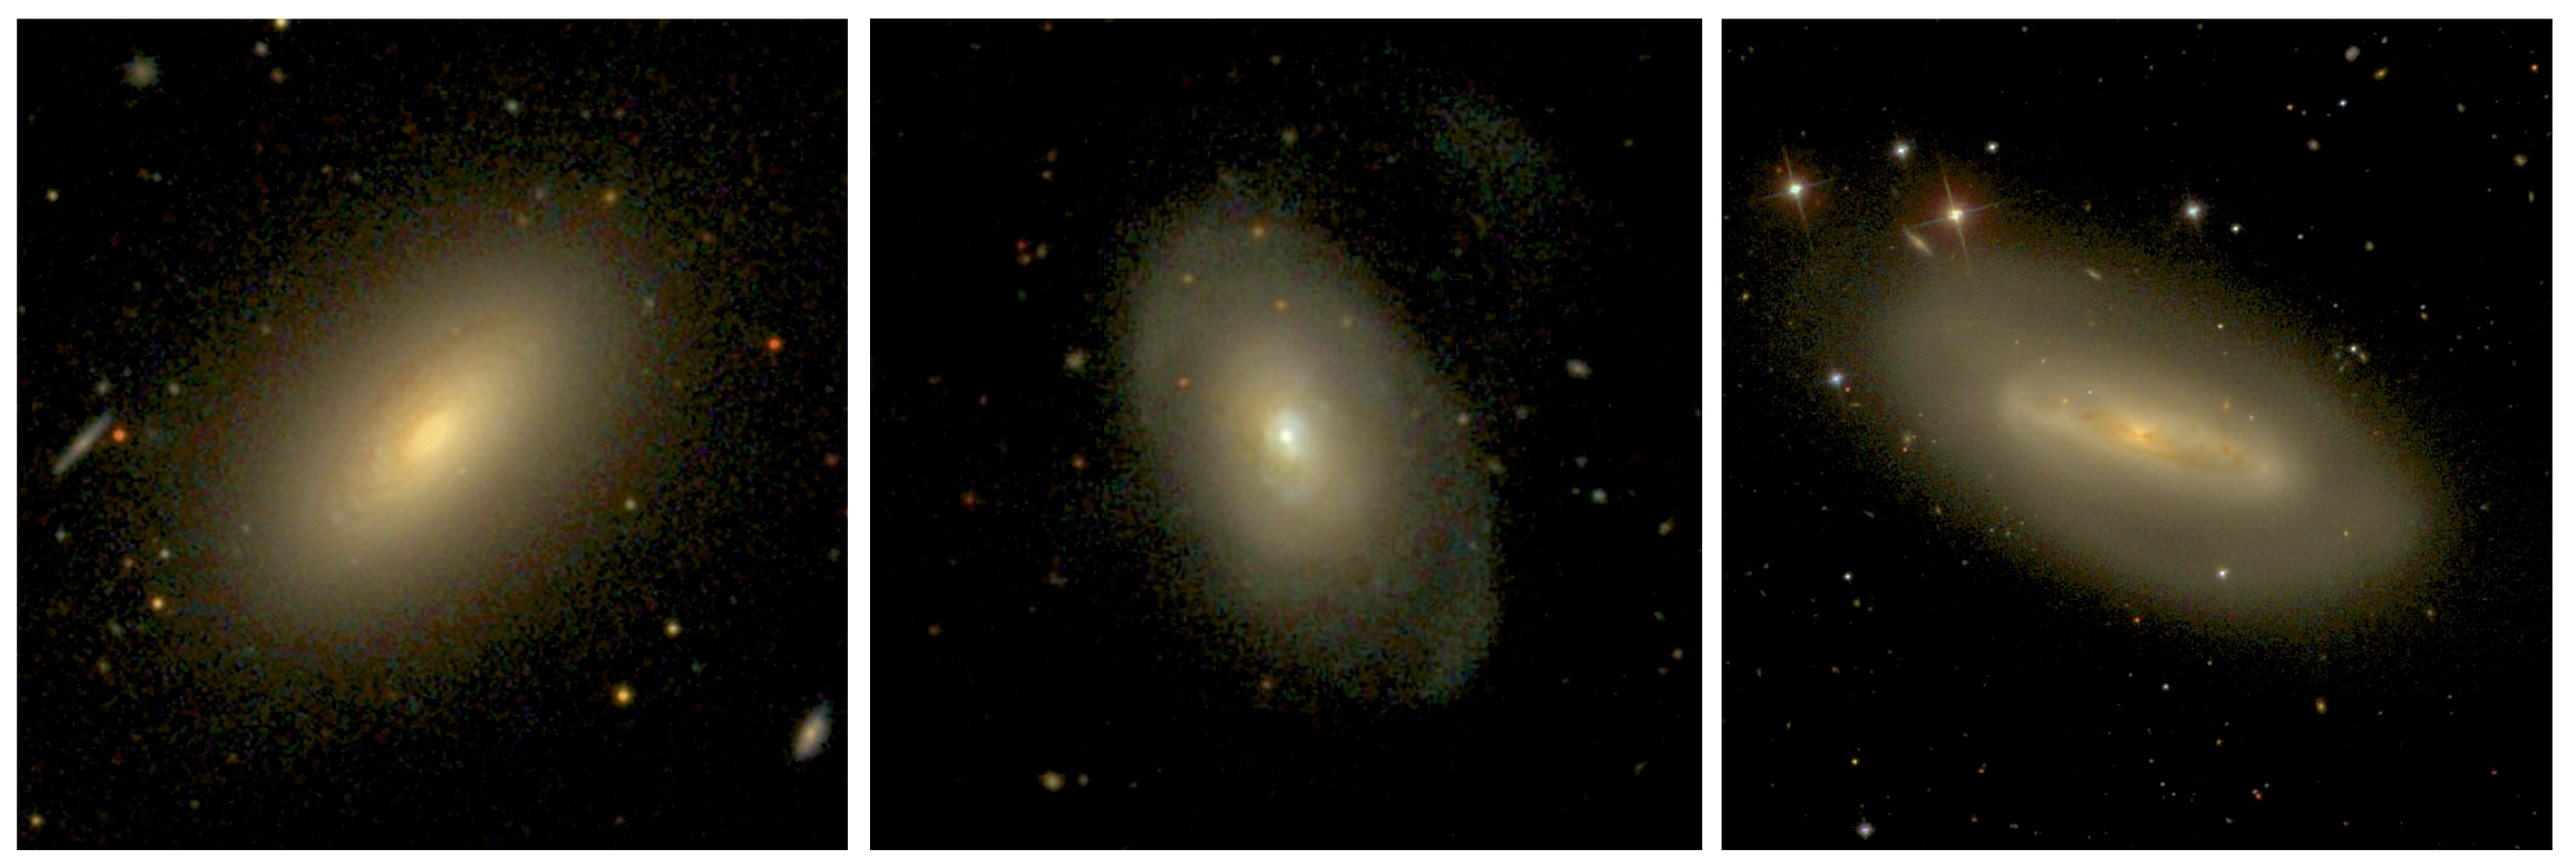
\includegraphics[width=84mm]{ExampleSas.png}
\caption{Examples of Sa galaxies with large, intermediate and small bulges from the classifications by Hogg, Roberts \& Sandage (1993).  The galaxies are (from left to right) large bulge Sa: NGC 2639; intermediate bulge Sa: NGC 3604; small bulge Sa: NGC 4293\label{Sa}}
\end{figure}

However modern automatic galaxy classification has tended to conflate bulge size alone with spiral type (e.g. Laurikainen et al. 2007, Masters et al. 2010a), and automatic classification of galaxies into ``early-" and ``late-" types, referring to their location on the Hubble Sequence and based on bulge-total luminosity ratio ($B/T$) or some proxy for this through a measure of central concentration, or light profile shape (e.g. Sersic index, as reviewed by Graham \& Driver 2005) has become common (e.g. van der Wel et al. 2011). Indeed, Sandage (2005) says this is not new, claiming "the Hubble system for disk galaxies had its roots in an arrangement of spirals in a continuous sequence of decreasing bulge size and increasing presence of �condensations� over the face of the image that had been devised by Reynolds in 1920."

It is clear that early S0 classification also included S0s with bulges of different sizes (S0a-S0c; Spitzer \& Baade 1951, van den Bergh 1976), a classification recently promoted by ATLAS-3D in their morpholology ``comb" which includes parallel sequences of star forming and passive (or aneamic) spirals, and a ETG fast-rotator bulge size sequence similar to the S0 sequence (Cappellari et al. 2011), as well as by Kormendy \& Bender (2012) in their parallel lenticular classification scheme explictly based on $B/T$. 

%Kormendy \& Bender (2012) present an update to a parallel lenticular classification scheme S0a-S0b-S0c first presented by van den Bergh (1976) and explicitly based on $B/T$ (since S0s by definition have no spiral arms). They extensively discuss S0c galaxies. 

It has also been understood for some time that the diversity of spiral arms observed in galaxies is not perfectly captured by the Sa-Sb-Sc spiral arm descriptors. As discussed at length by Buta (2012), the number of arms (commonly denoted $m$), ``character" of the arms (e.g. ``grand-design" or ``flocculent") and the sense of the winding of the arms relative to the galaxy rotation are all additional dimensions which can be used for classification (also see Elmegreen \& Elmegreen 1987, Ann \& Lee 2013). Buta (2012) notes that most low $m$ spirals are grand design, and goes on to discuss how spiral arm ``character" is thought to link to typical formation mechanism (with grand design spirals linked to density wave mechanisms, and flocculent spirals suggested to come from sheared self-propogating star formation regions). 

In this paper we will make use of Galaxy Zoo classifications, which provide a quantitative visual description of structures seen in local galaxies, capturing the typical range of descriptions used to construct the traditional Hubble sequence, but are not tied to any specific classification scheme (e.g. a spiral galaxy could be described has having tightly wound spiral arms and a large bulge, if this is how it looks). We'll review these classifications in Section \ref{sample}, give basic demographics of the local sample in Section \ref{demographics}, and discuss how to use them to construct a traditional Hubble sequence, along with the implications of trends of various visible structures in Section \ref{discussion}. We conclude with a Summary section. 

%Elmegreen \& Elmegreen 1987 - classes of spirals arms from flocculent to grand design.
%Discuss pseudo-bulges versus classical bulges (e.g. Fisher \& Drory)?


%In Hogg et al. 1993: recent discussions of the variation of physical parameters across the Hubble Sequence (e.g. Knapp et al. 1989, Eder et al. 1991, Young \& Scoville 1991). Discusses Sas with no evidence of star formation as being "generic to the classification sequence rather than the result of environmental processes (Sandage 1983)". 

\section{Sample and Data} \label{sample}

The first two phases of Galaxy Zoo (which ran from July 2007-April 2010\footnote{GZ1 is archived at {\tt http://zoo1.galaxyzoo.org}, and GZ2 at {\tt http://zoo2.galaxyzoo.org}}) were entirely based on imaging from the Legacy Survey of the Sloan Digital Sky Survey (SDSS; York et al. 2000). In this paper we make use exclusively of classifications from the second phase of Galaxy Zoo (or GZ2; Willet et al. 2013). In total, almost 300,000 images of galaxies were shown in GZ2, selected to represent the largest and brightest galaxies observed by SDSS. For full details of the sample selection see Willet et al. 2013, but in brief GZ2 made use of the SDSS DR7 imaging (Abazajian et al. 2009) and selected galaxies with $m<17.0$, $r>3\arcsec$ and $0.0005<z<0.25$ (or with no measured redshift). Image cutouts were generated as $gri$ colour composites centred on each galaxy with a size $8.48r_{90}\arcsec \times 8.48r_{90}\arcsec$, where $r_{90}$ is the radius containing 90\% of the r-band Petrosian aperture flux). 

Visual classifications for GZ2 were collected via a web interface, which presented volunteers with the colour cutout, and a selection of simple questions about the object shown. Following Willett et al. (2013) we define a {\it classification} as the sum of all information collected about a galaxy by a single user. These {\it classifications} are made up of answers to a series of {\it tasks} presented in a decision tree. A flow chart of this tree is presented as Figure 1 in W13, and for the convenience of the reader we reproduce Table 2 of W13 which summarizes all possible {\it tasks} and answers in Table \ref{tbl-tree}. 

\begin{table}
 \caption{The GZ2 decision tree, comprising 11 tasks and 37 responses. The `Task' number is an abbreviation only and does {\em not} necessarily represent the order of the task within the decision tree. The text in `Question' and `Responses' are displayed to volunteers during classification. `Next' gives the subsequent task for the chosen response. \label{tbl-tree}}
 \begin{tabular}{@{}cllr}
 \hline
\multicolumn{1}{l}{Task} &
\multicolumn{1}{c}{Question} &
\multicolumn{1}{c}{Responses} &
\multicolumn{1}{c}{Next} 
\\ 
\hline
\hline						
01    & {\it Is the galaxy simply smooth   }  & smooth           & 07 \\
      & {\it and rounded, with no sign of  }  & features or disk & 02 \\
      & {\it a disk?                       }  & star or artifact & {\bf end} \\
      \hline
02    & {\it Could this be a disk viewed   }  & yes              & 09 \\
      & {\it edge-on?                      }  & no               & 03 \\
      \hline
03    & {\it Is there a sign of a bar      }  & yes              & 04 \\
      & {\it feature through the centre    }  & no               & 04 \\
      & {\it of the galaxy?                }                                        \\
      \hline
04    & {\it Is there any sign of a        }  & yes              & 10 \\
      & {\it spiral arm pattern?           }  & no               & 05 \\
      \hline
05    & {\it How prominent is the          }  & no bulge         & 06 \\
      & {\it central bulge, compared       }  & just noticeable  & 06 \\
      & {\it with the rest of the galaxy?  }  & obvious          & 06 \\
      & {\it                               }  & dominant         & 06 \\
      \hline
06    & {\it Is there anything odd?        }  & yes              & 08 \\ 
      & {\it                               }  & no               & {\bf end}        \\
      \hline
07    & {\it How rounded is it?            }  & completely round & 06 \\
      & {\it                               }  & in between       & 06 \\
      & {\it                               }  & cigar-shaped     & 06 \\
      \hline
08    & {\it Is the odd feature a ring,    }  & ring             & {\bf end}        \\
      & {\it or is the galaxy disturbed    }  & lens or arc      & {\bf end}        \\
      & {\it or irregular?                 }  & disturbed        & {\bf end}        \\
      & {\it                               }  & irregular        & {\bf end}        \\  
      & {\it                               }  & other            & {\bf end}        \\  
      & {\it                               }  & merger           & {\bf end}        \\  
      & {\it                               }  & dust lane        & {\bf end}        \\  
      \hline
09    & {\it Does the galaxy have a        }  & rounded          & 06 \\
      & {\it bulge at its centre? If       }  & boxy             & 06 \\
      & {\it so, what shape?               }  & no bulge         & 06 \\
      \hline
10    & {\it How tightly wound do the      }  & tight            & 11 \\
      & {\it spiral arms appear?           }  & medium           & 11 \\
      & {\it                               }  & loose            & 11 \\    
      \hline
11    & {\it How many spiral arms          }  & 1                & 05 \\
      & {\it  are there?                   }  & 2                & 05 \\
      & {\it                               }  & 3                & 05 \\
      & {\it                               }  & 4                & 05 \\
      & {\it                               }  & more than four   & 05 \\
      & {\it                               }  & can't tell       & 05 \\
\hline
 \end{tabular}
\end{table}

W13 describes the process by which user responses are weighted and combined to provide vote fractions for each answer to each task for each galaxy in GZ2. We will refer to vote fractions as $p_{\rm xxx}$, where ``xxx" will describe the relevant answer. For example $p_{\rm features}$ will refer to the fraction of users answering {\it task} 01 by indicating they could see ``features or a disc" in the galaxy. W13 also describes a process of correcting for classification bias, caused primarilly by galaxies at larger redshift appearing dimmer and at coarser physical resolution than if viewed at lower redshift. Hart et al. (2016; hereafter H16) investigate this classification bias further, especially with regard to the visibility of spiral arms in GZ2, and update the redshift debiasing method to provide an updated set of debiased classifications from GZ2. In this paper we make use of the debiased classifications from H16, and when we use the terminology $p_{\rm xxx}$ we specifically refer to the debiased vote fraction. 

We select a low redshift volume limited sample, which is similar to the sample selection of (Hart et al. 2016, 2017). This is motivated by the desire to have galaxies with sufficient angular resolution that spiral arm features can be clearly identified and limit the impact of redshift debiasing. Of the {239,695} galaxies in GZ2 which have spectroscopic redshifts in DR7 (Abazajian et al. 2009, Strauss et al. 2002), we select $N=22,045$  galaxies which are found in the redshift range $0.01<z<0.035$, and which have an $r$-band absolute Petrosian magnitude of $M_r < -19.0$. We remove {six} of these galaxies which have more than 50\% of their classification votes for ``star or artefact". Inspecting these objects they are typically genuine galaxies, but with corrupted images (e.g. under a satellite trail, or diffraction spike from a nearby bright star). However, they do not have useful GZ2 classification since so many people marked them as artefacts.

``Features" in the Galaxy Zoo classification tree might include disturbed or irregular morphology or mergers. Users could identify these in GZ2 after indicating the that the galaxy showed ``odd" features, and then indicating what they thought was odd. All users classifying a galaxy answered this question. We select for these by requiring at $p_{\rm odd} > 0.42$ and $N_{\rm odd}>20$ (as recommended in W13), and then by requiring $(p_{\rm irregular}+p_{\rm disturbed} + p_{\rm merger} > 0.6$ (ie. approximately 60\% or more of the classifiers thought the galaxy was either irregular, disturbed or merging). As users could select only one of these options, using the sum is the most reliable way to identify all such objects. We find that {$N=1785$ (or 8\% of  the galaxies) meet these criteria, and of these 445 (2\%) are found to have the largest vote for ``merger", 137 (0.6\%)  for ``disturbed" and 1203 (5.4\%) for ``irregular"}. As these are a small fraction of the sample removing them makes little difference to the results below, never-the-less we remove them in what follows and proceed with {$N=20254$} ``normal" galaxies. 

We make use of Petrosian aperture photometry from SDSS in the urgriz bands. These are k-corrected as described in Bamford et al. (2009). Stellar masses are estimated from the colour-dependent mass-light ratio calibration presented by Baldry et al. (2009). $H_0$?

\section{Morphology of Local Galaxies} \label{demographics}

%We show in Figure \ref{sample}, the 22110 galaxies in our nearby volume limited sample on plots of $p_{\rm features}$ versus optical colour and magnitude ({\bf TODO: these are not the best way to get colour from SDSS, and also currently using DR7 not DR10}). These plots illustrate the well known tendency for galaxies to have two main morphological classes, in the GZ2 language those with features and those without, which is similar to the classic ``early-type" (meaning without spirals arms) and ``late-type" (\ie with spiral arms or other features). Note that the locus of ``featured" galaxies span the entire colour range of this volume limited sample, while ``smooth" galaxies are predominately red (although small samples of blue ``smooth" galaxies do exist, like the blue ellitpticals of Schawinski et al. 2009). 


\begin{figure*}
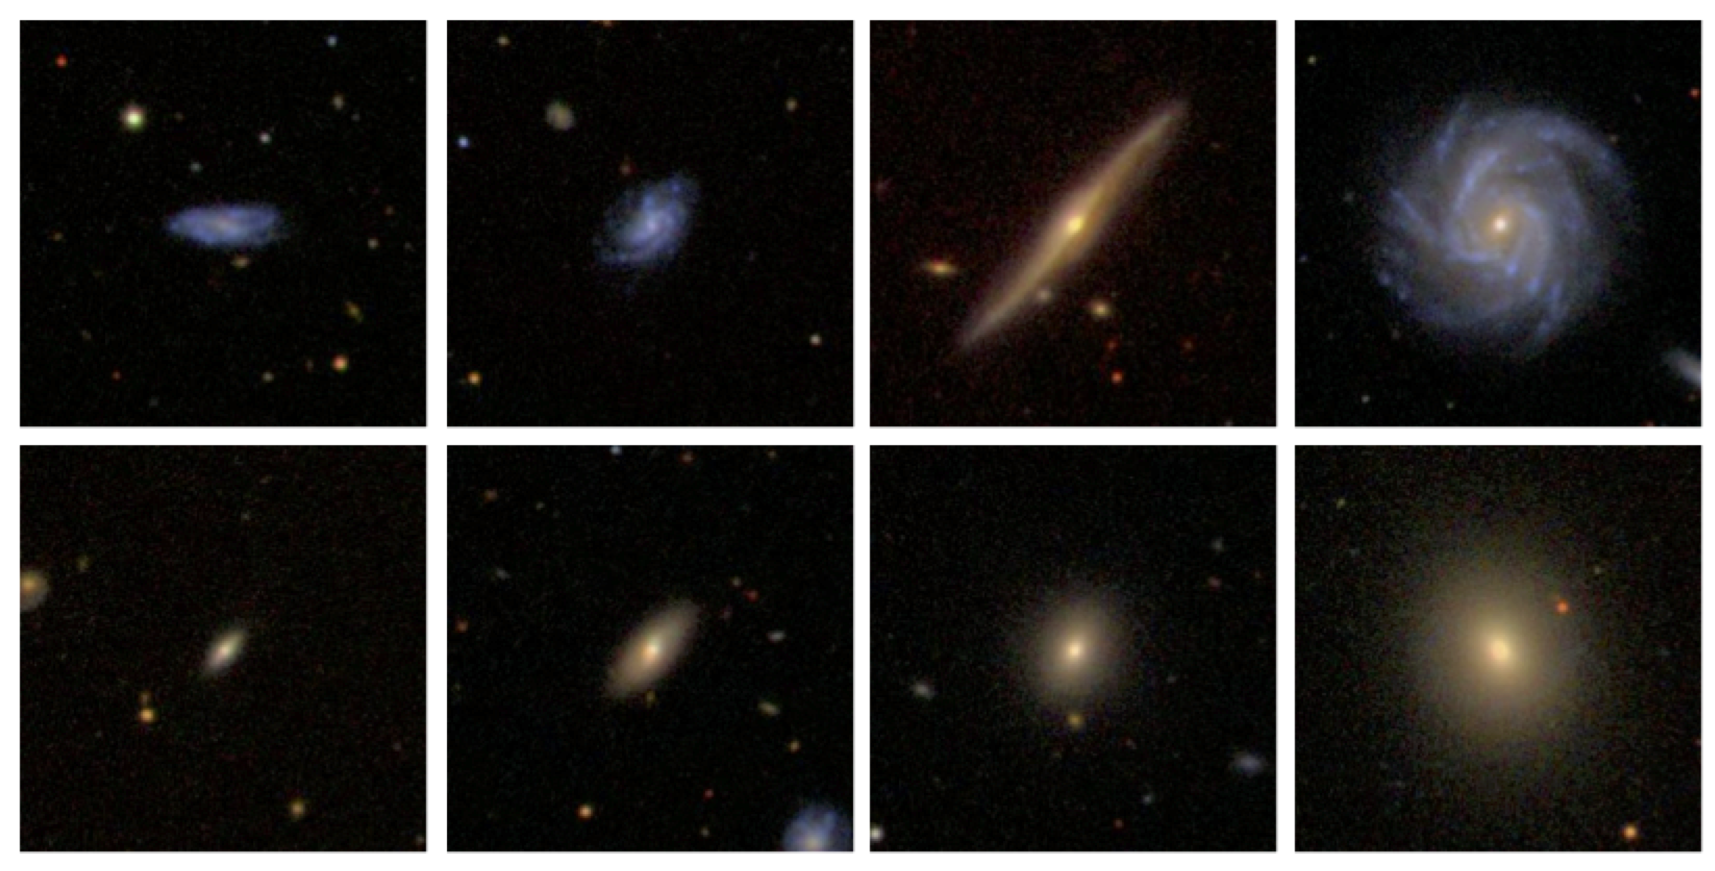
\includegraphics[width=160mm]{example1.png}
\caption{Randomly selected example images of galaxies classified as either ``featured" (top row) or ``smooth" (bottom row) from Galaxy Zoo as a function of $r$-band absolute magnitude (brighter to the right).  All galaxies have a redshift $z=0.03$ and are shown at the same angular scale. Images are $gri$ composites from SDSS with a scale of 1.7\arcmin square.  \label{examples}}
\end{figure*}


%\begin{figure*}
%\includegraphics[width=84mm]{barfraction_gasfraction.ps}
%\includegraphics[width=160mm]{sample_features.ps}
%\caption{Shown are plots of $p_{\rm features}$ versus absolute magnitude and optical colour, as well as a classic colour magnitude diagram for the 22118 galaxies in our nearby volume limited sample from Galaxy Zoo 2. This illustrated the known tendency for galaxies to have two main types split by both colour and magnitude. \label{sample}}
%\end{figure*}

 Many published works with Galaxy Zoo classifications use thresholds of $p_{\rm smooth}>0.8$ and $p_{\rm features}>0.8$ to identify cleanly classified galaxies. With these cuts, we find that {28\%} of galaxies in the sample are clearly ``featured", and {24\%} are clearly ``smooth", (the remaining 48\% have only lower consensus classifications; this can include genuinely intermediate type galaxies, but also any galaxy where volunteers did not have clear consensus on morphology). Relaxing these thresholds to rather use the majority answer for all galaxies in the sample allows every galaxy to be put into one category. With this cut (which is similar, but not identical to  $p_{\rm smooth}>0.5$ or $p_{\rm features}>0.5$, as well as the thresholds recommended in W13) we find {50\%} of the normal galaxies are best identified as ``featured" and {50\%} as ``smooth". Random examples of these two classes at $z=0.03$ (the median redshift of the sample) and as a function of absolute magnitude are shown in Figure \ref{examples}. % In Willet et al. (2013) we recommend thresholds of $p_{\rm smooth}>0.469$ and $p_{\rm features}>0.430$, with a minimum classifier count of $N=20$ to identify samples of galaxies in which classifications from further down the classification tree will  be reliable. We find 39\% of the sample ($N=8063$) pass this smooth threshold and 46\% ($N=9610$ pass it for featured), leaving 15\% ($N=3075$ galaxies) with only basic classifications. 
 Table \ref{basic} summarises these data, and in addition includes fractions for galaxies in subsets by their absolute magnitude which demonstrates the well known tendency for the brightest (or most massive galaxies) to be more likely to be ``smooth", although in this sample at similar rates to the lowest luminosity subsample. 
 
\begin{table*}
\caption{Distribution of basic morphological class\label{basic}. TODO: update numbers for final sample.}
\begin{tabular}{lccccc}
\hline\hline
Sample/defintion &  $N_{\rm smooth}$ & \%$_{\rm smooth}$ & $N_{\rm featured}$ & \%$_{\rm features}$\\
\hline
All ($N=20254$) \\
~~~~~~~~~ $ p>0.8$ & 4860 &  24 & 5694 &  28 \\
%~~~~~~~~~ $p>0.5$ & 7859 & 38 & 13069 & 63 \\
~~~~~~~~~ Majority vote & 10209 &  50 &  10045 & 50\\
%~~~~~~~~~ W13 criteria  & 8063 & 39 & 9610 & 46 \\
Majority vote  \\
~~~~~~~~~ Faint:  $M_r > -20$ ($N=9302$) & 5655 & 61 & 3647 & 39 \\
~~~~~~~~~ Mid 1:  $-21< M_r < -20$ ($N=7103$) & 2946 & 41 & 4157 & 58 \\
~~~~~~~~~ Mid 2:  $-22< M_r  < -21$ ($N=3408$) & 1349 & 40 & 2059 & 60 \\
~~~~~~~~~ Bright:  $M_r < -22$ ($N=441$) & 259 & 59 & 182 &  41\\
\hline\hline
\end{tabular}
\end{table*}


\subsection{Spiral Arms and Bars}
 
  It is only possible to identify spiral arms, bars and other disc features in disc galaxies which are sufficiently face-on for these to be visible. In a randomly oriented sample of disc galaxies, we expect to find $17\%$ of galaxies within $10\deg$ of perfectly edge-on. Among the galaxies identified as ``featured" in our ``normal" galaxy sample, we find {17\% ($N=1699$)} have values of $p_{\rm edge on}>0.8$. This is consistent with the number of galaxies expected to be found with $i\simeq90\deg$ in a randomly orientated sample of objects, which provides reassurance that the Galaxy Zoo "featured but not odd" sample is a reliable disc sample. W13 publish a recommended threshold for ``oblique" galaxies in which we can reliably identify disc features (e.g. bars, spirals) of $p_{\rm not edge on}>0.715$ (and $N_{\rm not edge on}>20$). In the sample discussed in this article, we find that {66}\% of the ``featured" galaxies fall into this group {($N=6614$)}. 
 
 Of these oblique featured galaxies: 
\begin{itemize}
\item {86}\% have clear spiral arms ($p_{\rm spiral} > 0.5$); just {5\%} are found to not have spiral arms to a high consensus ($p_{\rm spiral}<0.2$). 
\item {31}\% have obvious bars ($p_{\rm bar}>0.5$). This strong bar fraction is consistent with previous Galaxy Zoo based work (e.g. Masters et al. 2011, Masters et al. 2012), given the differences in sample selection. Weaker bars can be identified by $0.2<p_{\rm bar}<0.5$ (e.g. Willett et al. 2013, Skibba et al. 2011). Another {25}\% of the oblique spirals have weak bars by this definition, leaving just over {44\%} of oblique spirals without any clear sign of a bar feature (\ie~ $p_{\rm no bar}>0.8$) at the scales detectable by the SDSS images. 
\end{itemize}

Bars in GZ2 have been studied in many papers (e.g. Masters et al. 2010, 2012, Cheung et al. 2013, Galloway et al. 2016), and the number of spiral arms have been investigated by Willet et al. 2015, and most recently Hart et al. 2017. However to date there have been no publications making use of the identification of arm winding tightness from Galaxy Zoo. 

We define an arm winding score as
\be
\label{eqn:winding}
w_{\rm avg} = 0.0 ~p_{\rm loose} + 0.5 p_{\rm medium} + 1.0 p_{\rm tight}.
\ee
This has the advantage of providing a single number measuring the tightness of the spiral arms as seen by Galaxy Zoo users, and will be $w_{\rm avg} = 1.0$ where the arms are most tightly wound and $w_{\rm avg} = 0.0$ where they are very loose. We compare these identifications with pitch angles measured by the SpArcFiRe method (Hayes 2014) in Figure \ref{pitch}. This demonstrates how well arm winding as identified by Galaxy Zoo users correlates with pitch angle for those galaxies where pitch angle can be measured. The best fit trend gives 
\be
\label{eqn:pitch}
\Psi = 10.95 w_{\rm avg} + 14.73,
\ee
where $\Psi$ is the pitch angle in degrees, thus providing a way to estimate numerical pitch angles from the GZ2 visual descriptions. 

\begin{figure*}
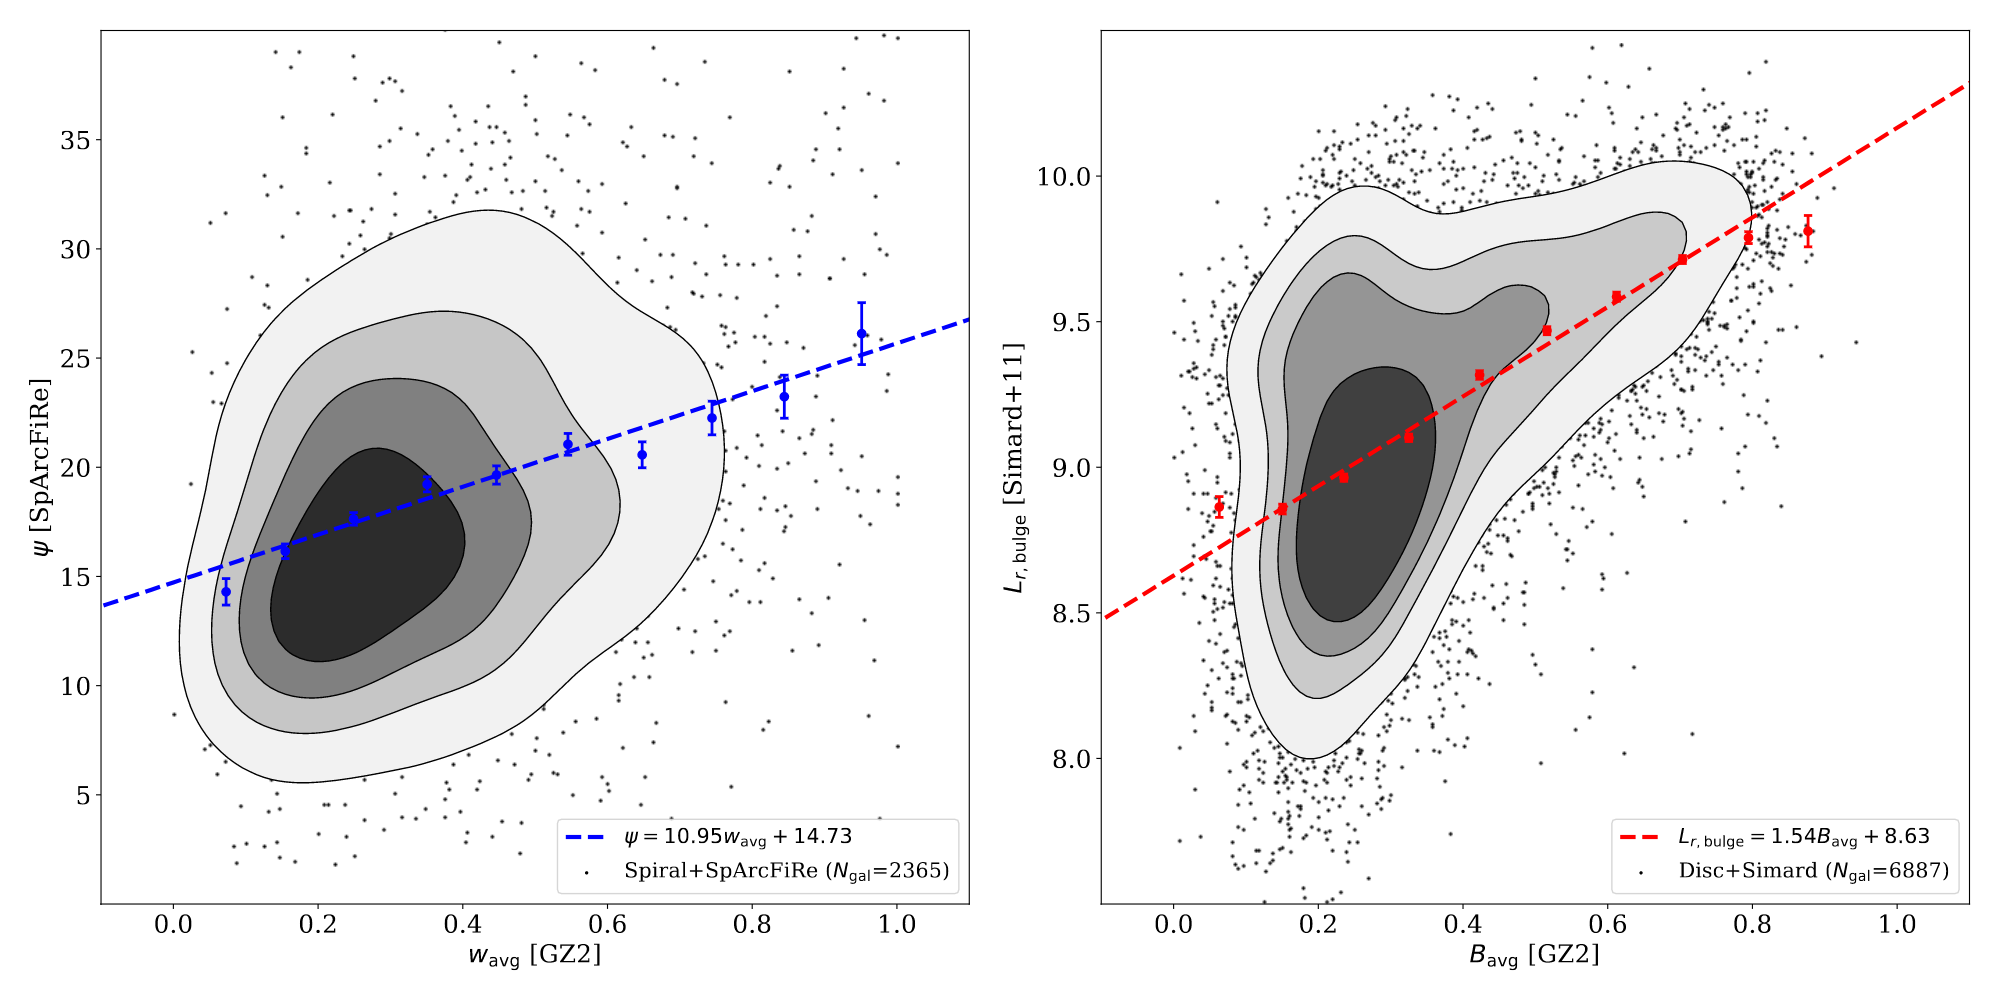
\includegraphics[width=140mm]{rossfigure.png}
\caption{(a) Galaxy Zoo winding score from Eq. \ref{eqn:winding} vs. measured pitch angles from SpArcFiRe for all spirals with at least one reliably identified arc (see Hayes 14 and Hart et al. 17). (b) Galaxy Zoo bulge prominence from Eq. \ref{eqn:bulge} vs. SDSS $r$-band bulge luminosity as measured from Simard et al. 2011. The grey contours indicate where 20, 40, 60 and 80\% of the galaxies lie in each plot and the dashed lines show the best fit straight line for each plot.  \label{pitch}}
\end{figure*}

We also plot on the right hand side of Figure \ref{pitch}, a measure of bulge size from GZ2 against the SDSS r-band luminosity of bulges as measured by Simard et al. (2011). The bulge prominence from GZ2 is defined as
\be
\label{eqn:bulge}
B_{\rm avg} = 0.0 ~p_{\rm no bulge} + 0.2p_{\rm  just} + 0.8p_{\rm obvious}+ 1.0~p_{\rm dominant},
\ee
again providing a single number, which ranges from $B_{\rm avg} = 0.0$ for galaxies with no bulge component, to $B_{\rm avg} = 1.0$ for spiral galaxies with completely dominant bulges. As can be see in Figure \ref{pitch} these two measures of bulge size correlate well, with a best fit of 
\be 
L_{\rm r,bulge} = 1.54 B_{\rm avg}  + 8.63.
\ee
 
 
% Examples of oblique galaxies with and without spiral arms and bars are shown in Figure \ref{examples2} for galaxies randomly selected from these groups at $z=0.03$. 
%\begin{figure}
%\includegraphics[width=84mm]{barfraction_gasfraction.ps}
%\includegraphics[width=80mm]{examplespiral_bar.ps}
%\caption{Examples of galaxies with (top row from left to right) $p_{\rm bar}>0.5$,  $0.2<p_{\rm bar}<0.5$ and $p_{\rm bar}<0.2$ and (bottom row from left to right) $p_{\rm spiral}>0.5$,  $0.2<p_{\rm spiral}<0.5$ and $p_{\rm spiral}<0.2$. The exact values of these debased classification fractions are indicated.   Images are $gri$ composites from SDSS with a scale of 1.7\arcmin square.  \label{examples2}}
%\end{figure}

\subsection{The Correlation of Bulge Size and Spiral Arm Tightness}

The classic Hubble Sequence for spiral galaxies implies that bulge size and spiral arm winding are highly correlated in most cases. In this section we investigate how tightly correlated bulge size and spiral arm tightness are found to be for galaxies with visible spiral arms in the Galaxy Zoo sample making use of the unique value of bulge size and spiral arm tightness from the GZ2 classifications as defined in Equations \ref{eqn:winding} and \ref{eqn:bulge}. These numbers increase from zero to one for either bulge sizes increasing, or arms getting tighter, in order than a ``classic" Sa should have both values of 1.0, and a ``classic Sc" would have both values of zero.  
 
 We plot the measure of bulge size versus arm windiness for the oblique spiral sample in Figure \ref{bulgewinding}. In this volume limited ($M_r<-19$) sample of nearby ($z<0.035$) galaxies we find no strong correlation between bulge size and arm windiness. There is a slight tendency spirals with large bulges to have only tightly wound spirals (\ie. both $A_{\rm winding}$ and $B_{\rm size}$ are large), but for spirals with small bulges all values of spiral arm winding are found.  This is consistent with the previous literature, in that Sa galaxies (as defined by arm winding) have been discussed with both large and small bulges, while Sc galaxies (as defined by loose arms) are only ever discussed with small bulges. 
 
 \begin{figure}
%\includegraphics[width=84mm]{barfraction_gasfraction.ps}
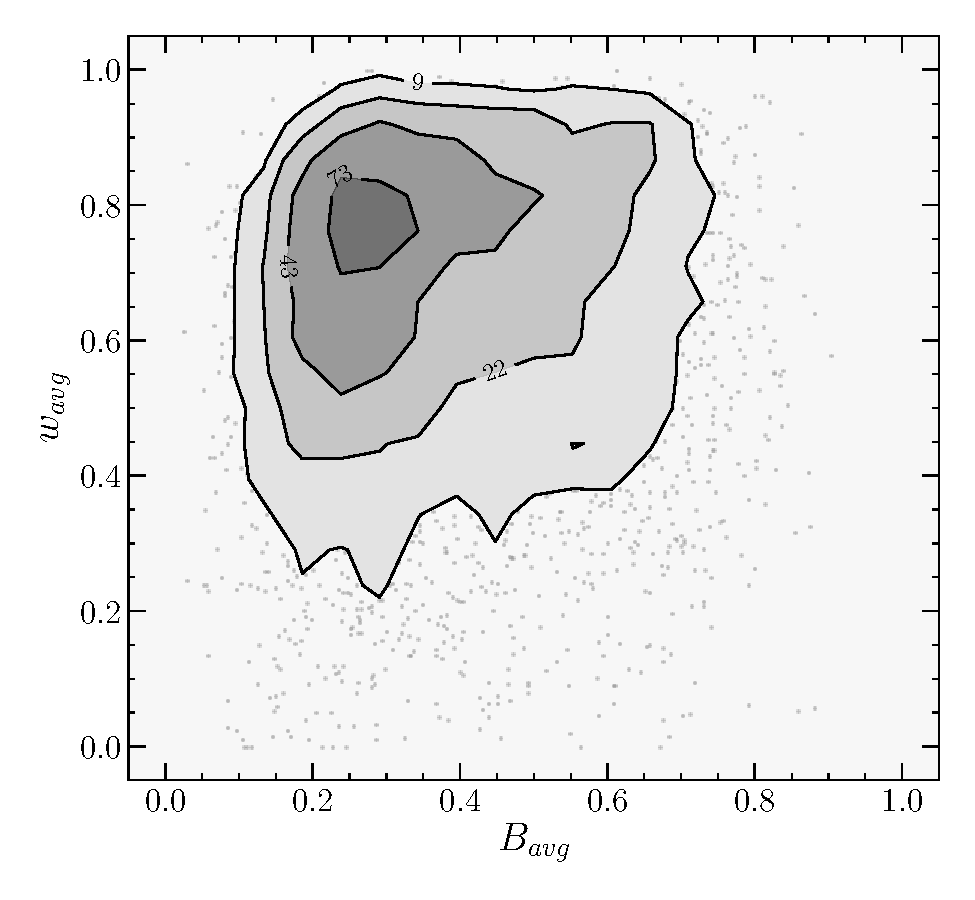
\includegraphics[width=80mm]{bulge_armwinding.pdf}
\caption{We show here the location of {4830} nearby spiral galaxies on a plot of bulge size versus degree of arm winding as indicated by Galaxy Zoo classifications. The contours indicate regions of high density, with the numbers showing the contour level value and points shown at the lowest density.   \label{bulgewinding}}
\end{figure}
 
 Given the traditional Hubble tuning fork is split by bar classification, we also split the sample based on the presence or absence of a strong bar. We find that spirals with strong bars ($p_{\rm bar}>0.5$)  were more likely to have larger bulges and less tightly wound spirals than those with no bars ($p_{\rm bar} < 0.2$), and for a given bulge size, barred spirals will have looser arms than unbarred spirals, but there remains no clear correlation between bulge size and spiral arm pitch angle in either subgroup (see Figure \ref{bars}). 
  
 \begin{figure*}
%\includegraphics[width=84mm]{barfraction_gasfraction.ps}
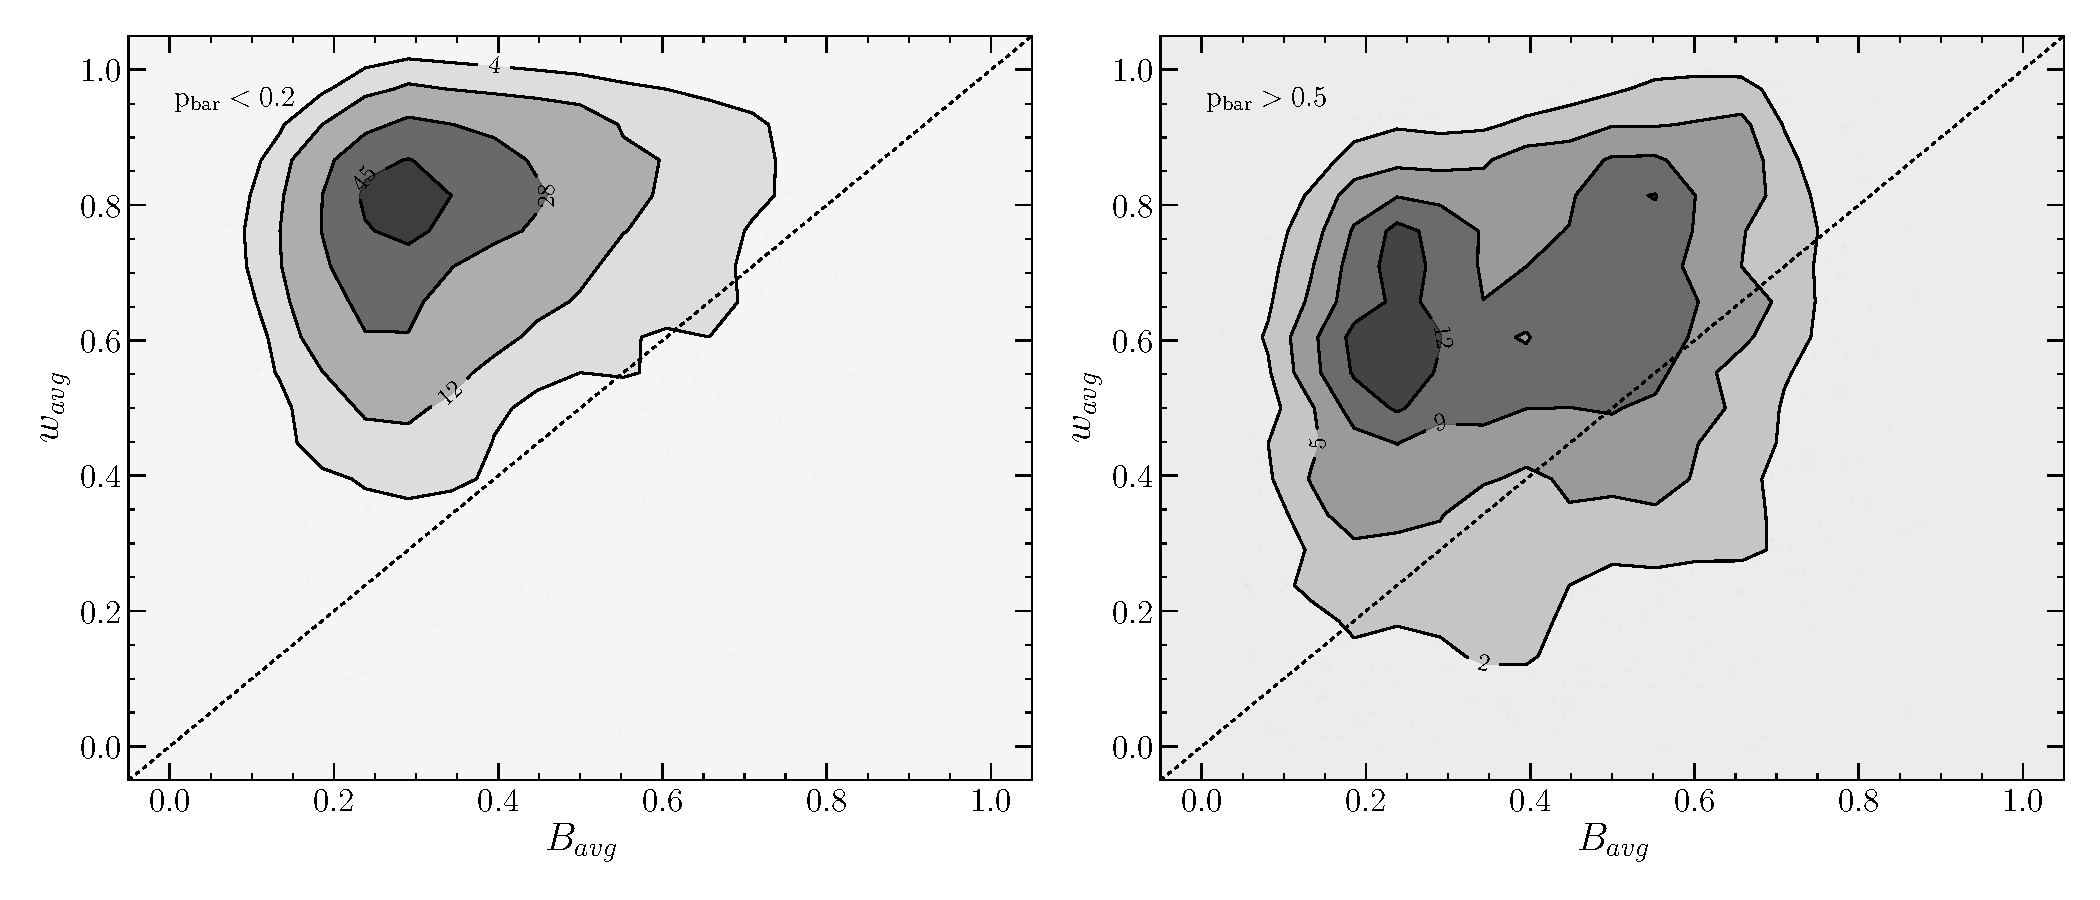
\includegraphics[width=160mm]{bulge_armwinding_split_bar.pdf}
%\includegraphics[width=80mm]{bulgewinding_bars.ps}
\caption{As Figure \ref{bulgewinding} but for subsamples of the oblique spirals split by bar classification.  Left panel: galaxies with $p_{\rm bar} < 0.2$; right panel: galaxies with $p_{\rm bar} > 0.5$ \label{bars}}
\end{figure*}

 Figure \ref{windingexample} shows examples of galaxies at $z=0.03$ from the four quadrants of Figure \ref{bulgewinding} with strong bars ($p_{\rm bar}>0.5$) or no bar ($p_{\rm bar} < 0.2$)
 
 \begin{figure*}
%\includegraphics[width=84mm]{barfraction_gasfraction.ps}
\center
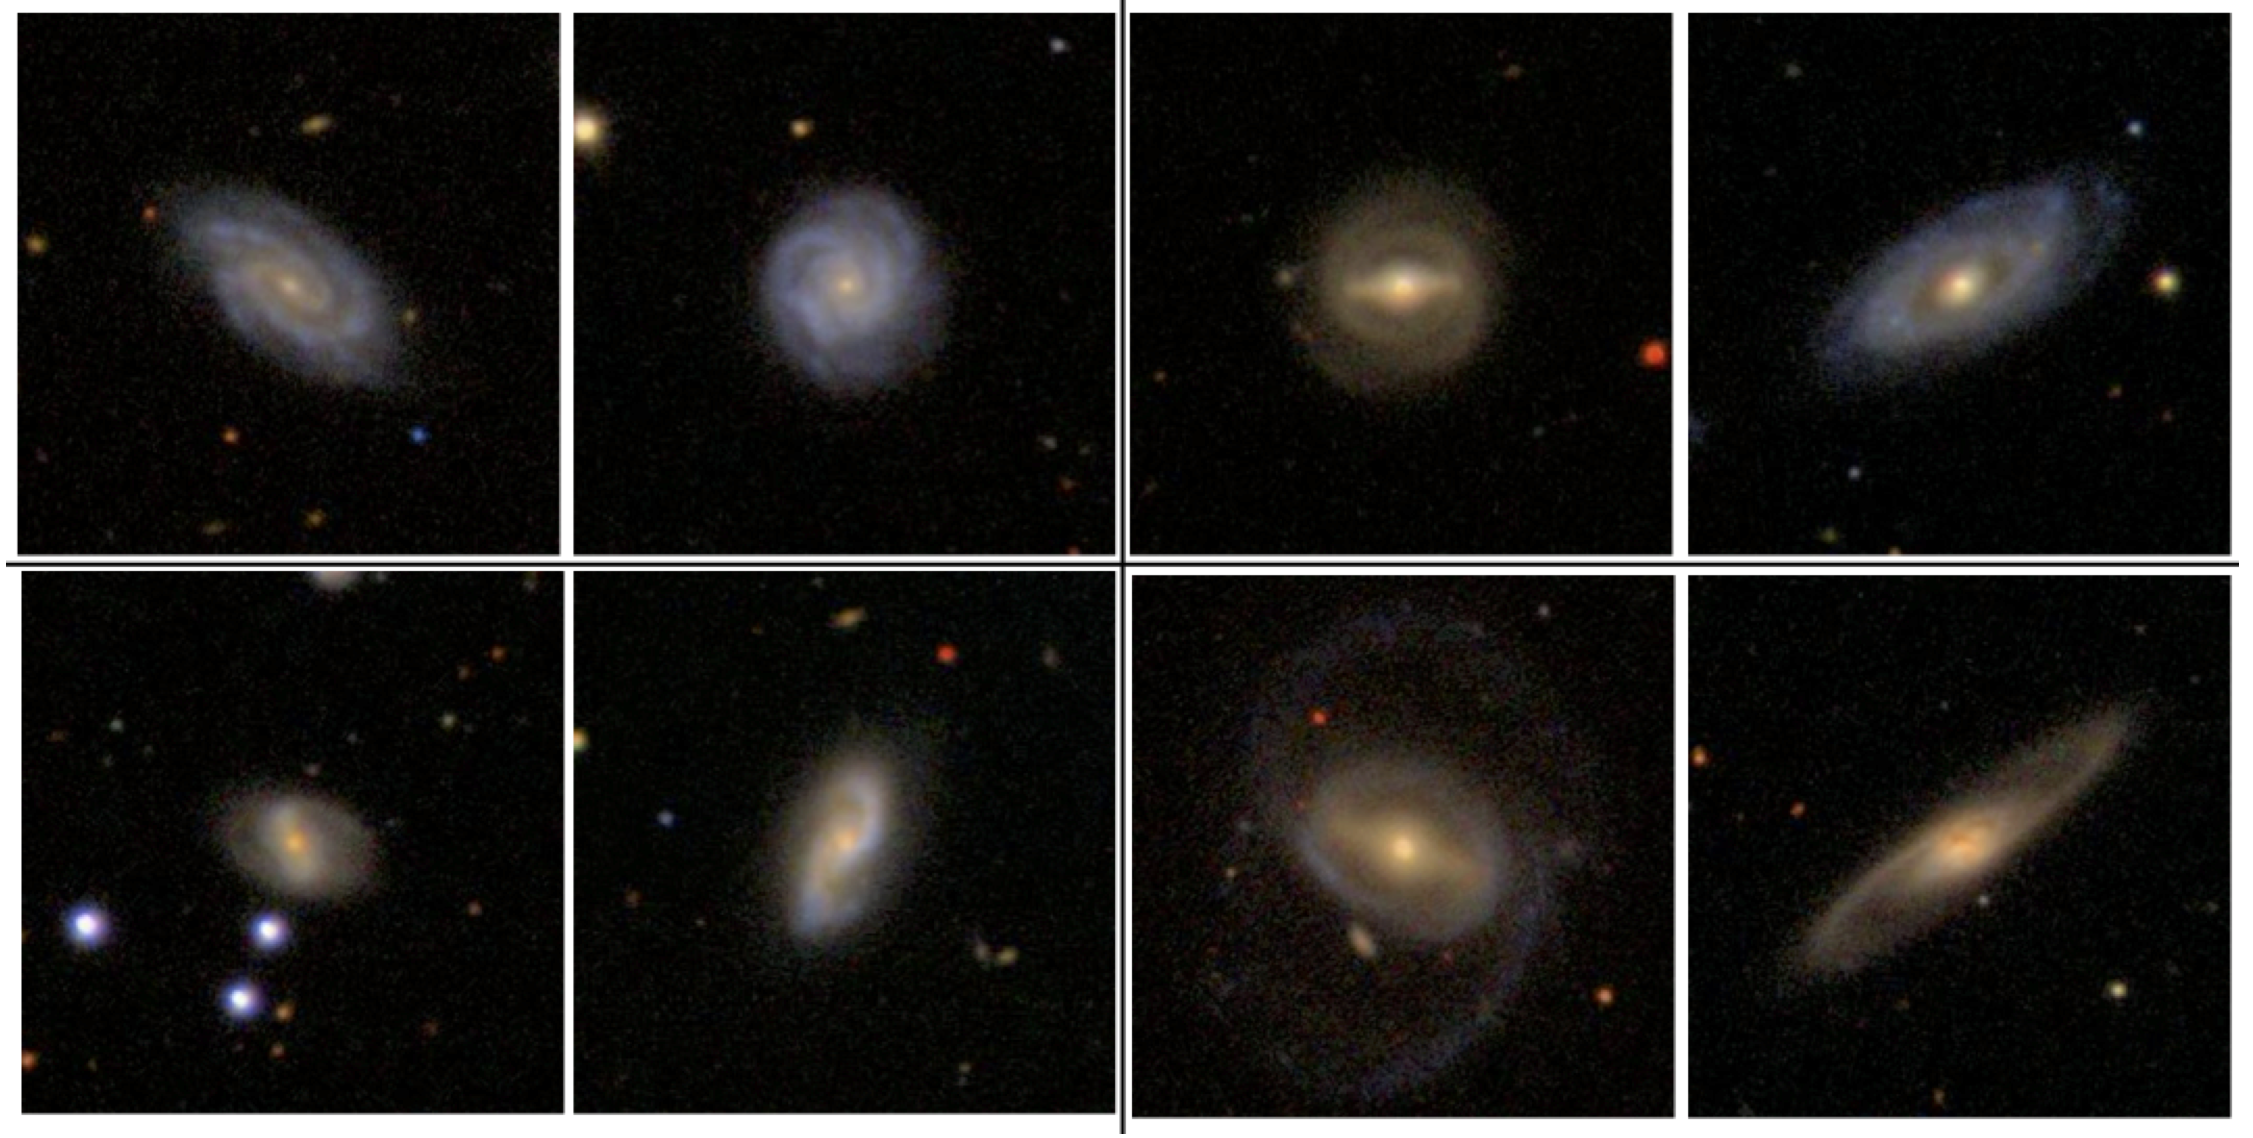
\includegraphics[width=160mm]{examplebulgewinding2.png}
\caption{Example images of galaxies at $z=0.03$ and $M_r\sim -21$ with both loose and tightly would spiral arms (lower and upper rows respectively) and small or large bulges (left and right columns respectively). In each case galaxies are shown with either strong bars, or no bar. Images are $gri$ composites from SDSS with a scale of 1.7\arcmin~ square.  \label{windingexample}}
\end{figure*}
 
\section{Discussion} \label{discussion}

% In this context we define a ``Hubble Sequence" as a sequence of galaxies in which the average physical properties vary systematically from ``early" (defined as low current star formation rates) to ``late" (defined as high current star formation rates). We consider optical colour as a proxy for SF (what about dust)..... 
 
 In W13 we discussed how best to assigned $T$-types to Galaxy Zoo galaxies from the classification votes in GZ2. Both the votes for tightness of spirals arms, and bulge size were considered. In that work we concluded that modern expert visual classification of spiral Hubble types (based on comparison with either Nair \& Abraham 2010, or Baillard et al. 2013) was primarily based on bulge size, regardless of the tightness of spiral arms, with the best fitting relation (based on symbolic regression) being found to be
 \be
 T = 4.63 + 4.17~p_{\rm no bulge} - 2.27~p_{\rm obvious} - 8.38~p_{\rm dominant}
 \ee 
 
We point the interested reader to the lower panel of Figure 19 from W13 which compares the predicted T-types from the above equation to the T-types assigned by Nair \& Abraham (2010). As was point out in W13, this, and other comparisons with recent expert visual classifications (e.g. the EFIGI sample of Baillard et al. 2011) demonstrates that the modern spiral Hubble sequence is defined by bulge size alone, with little reference to spiral arm tightness. 

%\begin{figure}
%\includegraphics[width=84mm]{barfraction_gasfraction.ps}
%\includegraphics[height=80mm,angle=-90]{T-typeW13.ps}
%\caption{Predicted T-type classifications as fit by Willett et al. 2013 for GZ2 galaxies shown versus their T-types from Nair \& Abraham 2010. Galaxies are colour coded by their morphologies as identified by NA10. Galaxies shown are only those with sufficient answers to characterize the arms winding and arms number GZ2 tasks, which selects heavily for late-type galaxies. This explains the lack of ellipticals in the plot, but highlights the fact that S0 galaxies do not agree well with the linear sequence. Reproduced from Willet et al. 2013.  \label{T-type}}
%\end{figure}

Models of spiral arm formation (see Dobbs \& Baba 2915 for a recent and comprehensive review) do not generally predict that spiral arm pitch angle should correlate with bulge size. For example, in swing amplification models, pitch angle should correlate best with spiral arm amplitude. In density wave models it should correlate best with the local shear in the disc (related to both disc mass, and the rotation speed - so total galaxy mass).  

Todo: write coherently something about what the pitch angle of spiral arms tells us physically and why we should care if it correlates with bulge size. 

From Hart et al 2016 "These properties are weakly related (Kennicutt 1981; Seigar \& James 1998): spiral arm tightness has been shown to be more strongly correlated with bulge total mass (Seigar et al. 2008; Berrier et al. 2013; Davis et al. 2015), rather than bulge-to-disk ratio."
"In particular, the pitch angle of spiral arms is related to both the star-formation rate in spiral galaxies (Seigar 2005), and the central mass concentration of the spiral galaxies (Seigar et al. 2006, 2014)."

From Dobbs \& Baba 2015  'Kennicutt (1981) indicates that the pitch angle correlates only in an average sense with galaxy type, and there is quite substantial spread.'



\section{Summary}

We present the morphological make-up of a sample of bright ($M_r <-19$), nearby ($0.01<z<0.035$) galaxies with classifications from the Galaxy Zoo project. We find that {92\%} of these galaxies show the ``normal" morphologies found on the classic Hubble sequence, with {8\%} classified as irregular, disturbed or merging. 

Among the ``normal" galaxies we find the typical correlation between magnitude, colour and morphology, such that ``smooth" (or ``early-type") galaxies are more common in the luminous red part of the diagram, where they make up ~50\% of the galaxies. Galaxies showing ``features" (or ``late-types") are found at all colours and magnitudes, and especially dominate the less luminous, bluer parts of the sample where they make up to two-third of the galaxies. 

 We find that the fraction of edge-on spirals is as expected for a sample of randomly orientated discs, and define a sample of ``oblique" spirals which are face-on enough for disc features to be identified. Among these {31\%} have strong bars, and {44\%} have no bars. The majority have clearly identified spirals ({86\%}), with only {5\%} with a clear consensus for lacking spiral arms. These are likely S0 types with rings or bars. 

Among the spiral galaxies, we find little or no correlation between spiral arm winding tightness and bulge size. Although spirals with large bulges are found to typically have tightly wound  arms, those with small bulges are found with a much wider range of spiral arm pitch angle. We find that the presence of a strong bar tends to correspond to more loosely wound arms and larger bulges. 

 We demonstrate that modern expert visual classification has moved away from the classic ``Hubble sequence" which prioritised spiral arm angles over bulge size (leading to discussion of small bulged Sa galaxies) and is now predominately an ordered on central bulge size. Something about how this makes sense for a sequence on star formation since bulge size correlates so well with star formation in discs...? 
 
  Some interpretation of what the degree of arm winding actually means. 
 
\paragraph*{ACKNOWLEDGEMENTS.} 

This publication has been made possible by the participation of more than 200,000 volunteers in the Galaxy Zoo project. Their contributions are individually acknowledged at \texttt{http://www.galaxyzoo.org/volunteers}. Galaxy Zoo 2 was developed with the help of a grant from The Leverhulme Trust.

We thank the contributors to the Galaxy Zoo Forum NGC Catalogue List \\(www.galaxyzooforum.org/index.php?topic=280028.0) for making finding SDSS images of NGC galaxies easy. 

Funding for the SDSS and SDSS-II has been provided by the Alfred P. Sloan Foundation, the Participating Institutions, the National Science Foundation, the U.S. Department of Energy, the National Aeronautics and Space Administration, the Japanese Monbukagakusho, the Max Planck Society, and the Higher Education Funding Council for England. The SDSS Web Site is http://www.sdss.org/. 

The SDSS is managed by the Astrophysical Research Consortium for the Participating Institutions. The Participating Institutions are the American Museum of Natural History, Astrophysical  Institute Potsdam, University of Basel, University of Cambridge, 
Case Western Reserve University, University of Chicago, Drexel University, Fermilab, the Institute for Advanced Study, the Japan 
Participation Group, Johns Hopkins University, the Joint Institute for Nuclear Astrophysics, the Kavli Institute for Particle Astrophysics and Cosmology, the Korean Scientist Group, the Chinese Academy of Sciences (LAMOST), Los Alamos National Laboratory, the Max-Planck-Institute for Astronomy (MPIA), the Max-Planck-Institute for Astrophysics (MPA), New Mexico State Uni- 
versity, Ohio State University, University of Pittsburgh, University of Portsmouth, Princeton University, the United States Naval Observatory and the University of Washington. 


\begin{thebibliography}{}
\bibitem[Ahn et al.(2013)]{2013arXiv1307.7735A} Ahn, C.~P., Alexandroff,  R., Allende Prieto, C., et al.\ 2013, arXiv:1307.7735 %DR10
\bibitem[Ann \& Lee(2013)]{2013JKAS...46..141A} Ann, H.~B., \& Lee, H.-R.\ 2013, Journal of Korean Astronomical Society, 46, 141 %Spiral arm morphology (by visual inspection of a few thousand SDSS images)
\bibitem[Baillard et al.(2011)]{2011A&A...532A..74B} Baillard, A., Bertin, E., de Lapparent, V., et al.\ 2011, \aap, 532, A74 
\bibitem[Buta (1992)]{B92} Buta, R. in {\it Morphological and Physical Classification of Galaxies}, ed. G. Longo, M. Capaccioli, G. Busarelo, p1, Dordrecht:Kluwer
\bibitem[Buta et al.(2007)]{BCO07} Buta, R.~J., Corwin, H.~G., \& Odewahn, S.~C.\ 2007, The de Vaucouleurs Altlas of Galaxies, edited by Ronald J.~Buta, Harold G.~Corwin and Stephen C.~Odewahn.~ISBN-13 978-521-82048-6 (HB).~Published by Cambridge University Press, Cambridge, UK, 2007.
\bibitem[Buta (2012)]{B12} Buta, R., 2012 in {\it Planets, Stars, and Stellar Systems} Vol 6. ed. W. C. Keel. 
\bibitem[Cappellari et al.(2011a)]{2011MNRAS.413..813C} Cappellari, M., et  al.\ 2011a, \mnras, 413, 813 
\bibitem[Cappellari et al.(2011b)]{2011MNRAS.416.1680C} Cappellari, M., Emsellem, E., Krajnovi{\'c}, D., et al.\ 2011b, \mnras, 416, 1680 
\bibitem[de Vaucouleurs (1956)]{dV56} de Vaucouleurs, G.\ 1959, Handbuch der Physik, 53, 275 
\bibitem[de Vaucouleurs et al. (1991)]{RC3} de Vaucouleurs, G., de Vaucouleurs, A., Corwin, H.~G., Jr., Buta, R.~J., Paturel, G., \& Fouqu{\'e}, P.\ 1991, Third Reference Catalogue of Bright Galaxies,~ Springer, New York, NY (USA).
\bibitem[Elmegreen \& Elmegreen(1987)]{1987ApJ...314....3E} Elmegreen, D.~M., \& Elmegreen, B.~G.\ 1987, \apj, 314, 3 %"Arm classifications for spiral galaxies"
\bibitem[Graham \& Driver(2005)]{2005PASA...22..118G} Graham, A.~W., \& Driver, S.~P.\ 2005, PASA, 22, 118 %Review of Sersic profiles
\bibitem[Hubble (1926)]{Hubble1926} Hubble, E., 1926, \apj, 64, 321 %Hubble classification
\bibitem[Kormendy \& Bender (2012)]{KB12} Kormendy, J., \& Bender, R. 2012, \apj SS, 198, 2. 
\bibitem[Lintott et al.(2008)]{L08} Lintott, C.~J., et al.\ 2008, \mnras, 389, 1179 %GZ1 description
\bibitem[Lintott et al.(2011)]{L11} Lintott, C.~J., et al.\ 2011, \mnras, 410, 166%GZ1 data
%\bibitem[Masters et al. (2010a)]{GZdust} Masters, K. L., et al. 2010a, \mnras ~404, 792. %dust %check number
\bibitem[Masters et al. (2010)]{M10} Masters, K. L., et al. 2010, \mnras ~405, 783.  %red spirals
%\bibitem[Masters et al. (2011)]{bars1} Masters, K. L., et al. 2011, \mnras . %bars
\bibitem[Nair \& Abraham(2010a)]{NA10a} Nair, P.~B., \& Abraham, R.~G.\ 2010a, \apj S, 186, 427 (NA10) %classifications
\bibitem[Park \& Choi(2005)]{2005ApJ...635L..29P} Park, C., \& Choi, Y.-Y.\ 2005, \apjl, 635, L29  %argues colour splits SDSS by morphology really well.
\bibitem[Roberts & Haynes (1994)]{RH9} Roberts, M. \& Haynes, M. 1994, \araa ~32, 115 %physical parameters along the Hubble Sequence
\bibitem[Sangage (1961)]{HubbleAtlas} Sandage, A., 1961, {\it The Hubble Atlas of Galaxies}, Washington: Carnegie Inst. Washington.
\bibitem[Sangage (1975)]{S75} Sandage, A. 1975. In {\it Stars and Stellar Systems}, Vol 9. ed. A. Sandage, M. Sandage, J. Kristian, p1, Chicago: Univ. Chicago Press.
\bibitem[Sandage (2005)]{S05} Sandage, A., 2005,\araa, 43, 581
\bibitem[Spitzer \& Baade(1951)]{1951ApJ...113..413S} Spitzer, L., Jr., \& Baade, W.\ 1951, \apj, 113, 413 %early investigation of S0s. 
\bibitem[Strateva et al.(2001)]{2001AJ....122.1861S} Strateva, I., et al.\ 2001, \aj, 122, 1861 %colour bi-modality
\bibitem[Strauss et al.(2002)]{MGS} Strauss, M.~A., Weinberg, D.~H., Lupton, R.~H., et al.\ 2002, \aj, 124, 1810 %SDSS Main Galaxy Sample.
\bibitem[van den Bergh (1976)]{vdB76} van den Bergh, S. 1976, ApJ, 206, 883
\bibitem[van den Bosch et al.(2008)]{2008MNRAS.387...79V} van den Bosch, F.~C., Aquino, D., Yang, X., et al.\ 2008, \mnras, 387, 79 %Satellite quenching in SDSS
\bibitem[van der Wel et al.(2011)]{2011ApJ...730...38V} van der Wel, A., Rix, H.-W., Wuyts, S., et al.\ 2011, \apj, 730, 38 %Using light profiles to classify galaxies
\bibitem[Weinmann et al.(2006)]{2006MNRAS.366....2W} Weinmann, S.~M., van den Bosch, F.~C., Yang, X., \& Mo, H.~J.\ 2006, \mnras, 366, 2  %discover of galactic conformity - late-type by colour/SFR. 
\bibitem[Willett et al.(2013)]{2013MNRAS.435.2835W} Willett, K.~W., Lintott, C.~J., Bamford, S.~P., et al.\ 2013, \mnras, 435, 2835 
\bibitem[Zehavi et al.(2011)]{2011ApJ...736...59Z} Zehavi, I., Zheng, Z., Weinberg, D.~H., et al.\ 2011, \apj, 736, 59  %SDSS MG clustering split by colour.
\end{thebibliography}

\end{document}
